\documentclass[../main.tex]{subfiles}

\begin{document}

\renewcommand{\labelitemi}{\ding{226}}
\renewcommand{\labelitemii}{\ding{227}}


\part{Introduction}
\label{part:intro:general}

\chapter{Neutrino physics}
\label{ch:nu_phys}
Exploration of the neutrinos is relatively young but perspective direction of the research in the particle physics. Over the last 60 years since its first experimental observation lots of breakthroughs were made. Many of them have been awarded with notable prizes. All this speaks of the great interest of the community in this topic. Many puzzles are still unsolved, plenty of challenging experiments are ongoing.

In this chapter the history of the neutrino research will be overviewed (\autoref{sec:hist}) as well as the current studies and experiments (\autoref{sec:exp}). The topic of the neutrino oscillations (\autoref{sec:osc}) will be described in more details as the main subject of the current thesis.

\section{Historical overview}
\label{sec:hist}
The prerequisites of the neutrino existence were found in the beginning if the XX century. The spectrum of the electrons from the neutron decay (called $\beta$-decay) was measured as continuous but not discrete~\cite{Chadwick1914}. At that time the neutron decay was imagined as $n\to p+e$. Non-discrete spectrum provoked plenty of theories such as energy non-conservation (by N. Bohr) or existence of the new hypothetical particle (by W. Pauli~\cite{Pauli1930}). Later Enrico Fermi developed a complete theory of the beta decay~\cite{Fermi1934}. In the modern notation the decay process was presented as $n\to p^++e^-+\overline{\nu}_e$. Where neutrino is noted as $\nu$.

\subsection{Discovery of the neutrino}
The experimental discovery of the neutrino was pretty challenging. Neutrinos are not taking part in the electromagnetic or strong interactions. The only way to detect them is a weak interaction. Based on the Fermi's theory the inverse beta decay process should exist that will allow the direct observation of the neutrino. But the expected cross-section for such process was estimated at the level of $10^{-44} cm^2$. That was about couple of dozen orders less then cross-sections of the processes that were usually observed in the experiments at that time. That's why the neutrino discovery happened only 26 years after the proposal of the new particle.

After the proposal of the new particle few indirect measurements were performed, but the direct observation still remained a challenge. The first successful neutrino detection were done by group leading by Frederick Reines and Clyde Cowan~\cite{Cowan1956}. They performed series of experiments trying to detect neutrino from the most powerful source at that time - nuclear power plant. Relatively brand new material a liquid scintillator was used as a target and detector. The inverse beta decay was used as a detection reaction:
\begin{equation}
\bar{\nu}+p\to n+e^+
\end{equation}
The positron shortly annihilates with emitting of photons. In order to suppress background the Cadmium isotope was added to the detector. Thus the neutrons would be also detected with reaction
\begin{equation}
n+{}^{108}Cd\to{}^{109m}Cd\to{}^{109}Cd+\gamma
\end{equation}
As the ${}^{109m}Cd$ lifetime is few tens microseconds the signal will have the unique signature: positron annihilation, and after a known time delay the gamma ray emission. Both signals will come with the fix energies. Thus rare signal events could be easily separated from the variety of the backgrounds.

Such strategy lead to the successful discovery of the particle that supposed to be ``undetectable'' before.

\subsection{Neutrino and anti-neutrino}
\label{sec:anti}
Soon after the neutrino discovery the question of its equivalence with the anti-neutrino was risen. Neutrino was the only known fermion without electric charge. So it was the only candidate for such equivalence. Raymond Davis performed the attempt to detect neutrino interactions with induction either electron or positron~\cite{Davis1955}. He used a clear beam of anti-neutrinos from the reactor. If both reactions~\autoref{eq:nu} and~\autoref{eq:antinu} were detected that would mean that the neutrino ant anti-neutrino are equal.

\begin{eqnarray}
\label{eq:nu}
\bar{\nu}+p\rightarrow n+e^+ \\
\nu+n\rightarrow p+e^-
\label{eq:antinu}
\end{eqnarray}

He used the nuclear reaction with chlorine proposed by the Pontecorvo $\nu+{}^{37}Cl\to e^-+{}^{37}Ar$ with further decay of the ${}^{37}Ar$ with $\tau_{1/2}=35$ days. Such reaction was not observed that meant that neutrino interacted in different way comparing to anti-neutrino.

Goldhaber performed other extremely interesting experiment trying to measure the neutrino helicity~\cite{Goldhaber1958}. The electron capture by the Europium atom was used. The produced excited atom of Samarium further decay with photon emission. The photon polarity strictly depends on the neutrino helicity, that's how the last could be measured.

\begin{align}
Eu+e^-\to\nu+&Sm^* \\ \nonumber
&Sm^*\to Sm+\gamma
\end{align}

Goldhaber found that neutrino has only left helicity.

\begin{bclogo}[couleur=blue!2, arrondi=0.1, logo=\bcinfo, nobreak=true]{Helicity, polarity, chirality}
Helicity is a projection of the spin onto the direction of the momentum.
\begin{equation}
h=\frac{\vec{s}\cdot\vec{p}}{\left|\vec{s}\right|\left|\vec{p}\right|}
\end{equation}

The helicity could be ``left'' or ``right'' that corresponds to the spin direction opposite or co-directed with momentum. For the massless particles helicity is Lorentz invariant. The polarization of the particle beam is a percentage of the particles with a given helicity. For example 50\% polarization means that half of the particles are ``left'' and half are ``right''.

The chirality is a more fundamental characteristic versus helicity. It is determined by whether the particle wave function transforms with a right- or left-handed representation of the Poincare group.

Massless fermions keep chiral symmetry, i.e. independent rotation of the left- and right- handed components doesn't affect the theory. For them the helicity is always the same as chirality.

The massive particles break the chiral symmetry explicitly. Also for the massive fermions helicity is never more equivalent to the chirality as one could choose the reference frame moving faster then the particle and inverse the helicity.
\end{bclogo}

Combining results from Davis and Goldhaber we could conclude that neutrino and anti-neutrino interact in the different way, their helicity is different. Thus we still have possibility to describe the neutrino and anti-neutrino as the same particle but with different helicity. Such formalism was developed long before the described experiments by Ettore Majorana~\cite{Majorana1937}. He found a particular solution of the Dirac equation.

\begin{equation}
\left(i\gamma^\mu\partial_\mu-m\right)\psi=0
\end{equation}

In particular case of fermions the particle could be described in terms of spinors

\begin{align}
i\gamma^\mu\partial_\mu\psi_L&=m\psi_R\\ \nonumber
i\gamma^\mu\partial_\mu\psi_R&=m\psi_L
\end{align}

In case of massless fermion, like neutrino in the Standard Model (\autoref{sec:sm}) such notation is called Weyl spinors with two components. If the fermion is massive it could be described with four component spinors but only if $\psi_L$ and $\psi_R$ are dependent. That's how the Majorana equation was obtained

\begin{equation}
i\gamma^\mu\partial_\mu\psi_L=m\mathcal{C}\bar{\psi_L}^{T}
\end{equation}

This equation works only in case $\psi=\psi^C$. It means that such approach is not suitable for any charge fermion as their charge conjugation states are different because of e.g. different electric charge. But the neutrino is a unique particle to which this approach may be applicable.

Is neutrino a Majorana fermion or a Dirac fermion is still an open question. Neutrino oscillation experiments are not sensitive to this difference. The only way at the moment to find if the neutrino is a Majorana fermion is to detect the neutrinoless double beta decay. Plenty of experiments are challenging in this study~\cite{Bilenky2015}.

\begin{bclogo}[couleur=blue!2, arrondi=0.1, logo=\bcinfo, nobreak=true]{Symmetries: C, P, T}
In particle physics there are three important symmetries: charge (C), parity (P) ant time (T).

Parity inversion (P) flip the sign of the spatial coordinate $\mathcal{P}\overrightarrow{r}=-\overrightarrow{r}$ . In the QFT it's described as $\mathcal{P}\lvert\psi\rangle=c\lvert\psi\rangle$. Where $c$ is the eigenvalue of $\mathcal{P}$. The parity violation means a process that change the eigenvalue of the parity transformation for some system. The theory of such process was developed by Lee and Yang~\cite{Lee1956} and found in the Wu's experiment~\cite{Wu1957}. The asymmetry of the outgoing electrons from the Cobalt with respect to the nucleus polarization was the nice and clear proof for the effect.

Charge symmetry (C) transform particle to its anti-particle. $\mathcal{C}\lvert\psi\rangle=\eta_{C}\lvert\bar{\psi}\rangle$, where $\eta_{C}$ is the eigenvalue of the transformation. The example of the eigenvalue non-conservation experimental observation could be found in~\cite{Gormley1968}.

Time transformation (T) inverse the time direction. After the discovery of the separate P and C violations the combined symmetry breaking became the puzzle.

As it will be a hint towards T-symmetry breaking. The CP-violation was observed in the neutral kaons oscillations process~\cite{Christenson1964}. Later such process was confirmed with the direct measurements of kaon decays~\cite{AlaviHarati1999}~and~\cite{Fanti1999}, B-meson decays~\cite{Aubert2001}~and~\cite{Abe2001}, D-mesons~\cite{Aaij2019}.

Together they form a CPT symmetry. It's proved that any Lorentz invariant local quantum field theory with a hermitian Hamiltonian must be invariant under CPT.
\end{bclogo}


\subsection{Different types of neutrino}
\label{sec:dublet}
The first neutrino detection was made using the reactor as a particle source. Such source is extremely powerful, but isotropic. For the precise measurements is will be extremely useful to gain the statistics with the focused particle beam. For this the accelerators could be used. The general idea is to use proton beam hitting the target for the massive meson production. The charged meson could be focused and further decay producing the focused neutrino beam with high intensity. The description of such scheme in the modern experiment could be found in~\autoref{ch:T2K:nu_beam}. First time such approach was used to determine if the neutrino has flavors~\cite{Danby1962}. The main idea of the experiment is to use the neutrino flux produced from the pion decay. Because of the mass difference between electron and muon and the fixed neutrino helicity (\autoref{sec:anti}) charged pion decays mainly to muon, e.g. $\pi^+\to\mu^++\nu$. The question is could neutrino be ``muon'' or ``electron''. The experiment showed clearly that the reaction~\autoref{eq:notallowed} is severely suppressed comparing the reaction~\autoref{eq:allowed}.

\begin{align}
\label{eq:allowed}
\nu_\mu+p&\rightarrow n+\mu \\
\nu_\mu+p&\nrightarrow n+e
\label{eq:notallowed}
\end{align}

That means that neutrino has flavors. It could be either produced or detected with the lepton of the same flavor. The existence of the different types of the neutrino confirmed the doublet structure of the leptons. This fact will play an important rope in the theory of the neutrino oscillations.


\subsection{Neutrino in the Standard Model}
\label{sec:sm}

The first step towards the general model of particle physics was done by Yang and Mills with extending of the concept of the gauge theory to the nonabelian groups. This made possible to describe the phenomena of strong interactions~\cite{Yang1954}. Later Glashow found a way to unify the electromagnetic and weak interactions~\cite{Glashow1961}. Salam and Weinberg finished the theory with implementation of the Higgs mechanism into the Glashow theory~\cite{Weinberg1967}.

Plenty of experiments brilliantly confirmed the proposed model and demonstrated its incredible predictive power. For example in the part of the electroweak interactions the most breakthrough observations were: neutral current discovery~\cite{Cundy1974}, Z and W boson discovery~\cite{Arnison1983}, $\gamma-Z$ interference, neutrino generation number~\cite{Arnison1983}, Higgs boson discovery~\cite{Aad2012}, and many others.

The schema describing the Standard Model is presented on~\autoref{fig:intro:SM}.

\begin{figure}[!ht]
    \centering
    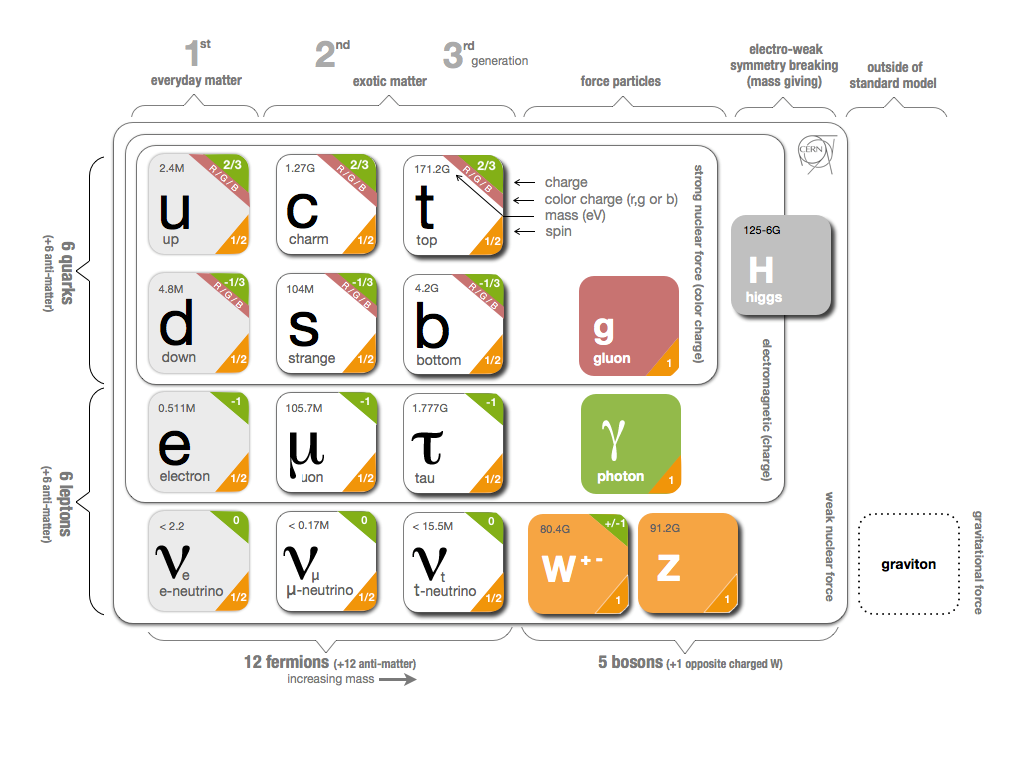
\includegraphics[width=0.8\linewidth]{SM.png}
    \caption{A schematic view of the Standard Model (SM) of the particle physics.}
    \label{fig:intro:SM}
\end{figure}

In general the SM is based on the Yang–Mills theory with local $SU(3)\times SU(2)\times U(1)$ gauge symmetry. It could be divided into several parts:
\begin{itemize}
  \item Quantum chromodynamics sector
  \item Electroweak sector
  \item Higgs sector
  \item Yukawa sector
\end{itemize}

In context of current thesis the electroweak sector is the most interesting. It is based on the group $U(1)\times SU(2)_L$. It mean that we well have two generators: the weak hypercharge ($Y_W$) for $U(1)$ and Pauli matrices for $SU(2)_L$. Index $L$ mean that it affects only left-chiral fermions.

In the SM fermions are described as a doublets (\autoref{sec:dublet}). For each charged lepton there is an appropriate neutrino. While charged lepton could be either right-handed or left-handed, the neutrino could be only left-handed. This part of theory is based on the empirical observations (\autoref{sec:anti}) and this is strictly fixed in the model. Neutrino could interact with the charge current (CC) or neutral current (NC). The appropriate interaction terms are defined as:

\begin{align}
-\mathcal{L}_{CC}&=\frac{g}{2}\sum_\alpha\bar{\nu}_{L\alpha}\gamma^\mu\ell_{L\alpha}W^+_\mu+h.c. \\ \nonumber
-\mathcal{L}_{NC}&=\frac{g}{\sqrt{2\cos{\theta_W}}}\sum_\alpha\bar{\nu}_{L\alpha}\gamma^\mu\nu_{L\alpha}Z^0_\mu
\end{align}

Thus there is no chance for production or detection of the right-handed neutrino (left-handed anti-neutrino).

\subsection{Neutrino flavors}
After the magnificent confirmation of the Standard Model with discovery of the neutral current and W and Z bosons, it became possible to measure precisely the number of neutrino generations. This analysis became possible with massive production of the Z-bosons on so-called Z-factory such as Large Electron-Positron Collider (LEP) at CERN.

The general idea of the study is to look at the different modes of the Z decays. All the decays could be classified into several groups:

\begin{align}
Z&\to hadrons \nonumber \\
Z&\to \ell^+\ell^- \\
Z&\to \nu\bar{\nu} \nonumber
\end{align}

The total width of the boson decay sums up from these three parts. As width of $Z\to \ell^+\ell^-$ is the same of all charge leptons and $Z\to \nu\bar{\nu}$ is the same for all neutrino types they could be multiplied with an appropriate number:

\begin{equation}
\Gamma_Z=\Gamma(Z\to hadrons)+N_{\ell}\times\Gamma(Z\to \ell^+\ell^-) + N_{\nu}\times\Gamma(Z\to \nu\bar{\nu})
\label{eq:intro:nnu}
\end{equation}

During the experiment the $\Gamma_Z$, $\Gamma(Z\to hadrons)$ and $\Gamma(Z\to \ell^+\ell^-)$ were measured. The equality of the $\Gamma(Z\to e^+e^-)$ and $\Gamma(Z\to \mu^+\mu^-)$ was checked. The width of the decay into neutrons came from the theory. The number of neutrino generations remained the only unknown variable in the~\autoref{eq:intro:nnu}. The results of the precise measurements of the Z-boson resonance and predictions for 2, 3 and 4 neutrino generations are shown in~\autoref{fig:intro:NuGen}. From these studies the $N_{\nu}=2.9840\pm0.0082$. So we could conclude that there are only three types of the left-handed neutrino with masses less than Z-boson mass.

\begin{figure}[!ht]
    \centering
    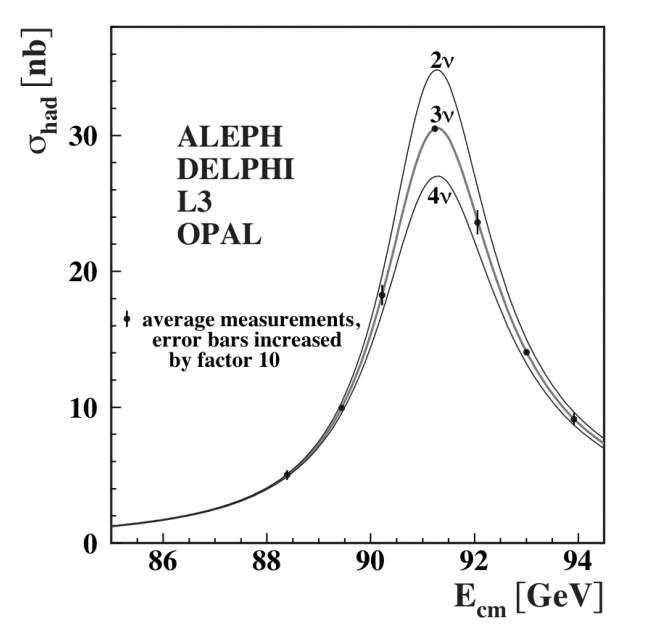
\includegraphics[width=0.6\linewidth]{Neutrino_gen.png}
    \caption{Measurement of the hadron production cross-section as a function of the LEP center-of-mass energy around the Z-boson resonance.}
    \label{fig:intro:NuGen}
\end{figure}


\subsection{Neutrino mass measurements}
In spite of the Standard Model assumption about the neutrino massless nature there were plenty attempts to measure its mass. After the confirmation of the fact that neutrino has mass from neutrino oscillation phenomena (\autoref{sec:osc}) these measurements became essential.

\subsubsection{Beta decay}
The straight-forward way for the neutrino mass measurements is a search for the effect of the nonzero neutrino mass in the beta decay spectrum. One need to measure the energy of outgoing electrons and look at the far end of the distribution. The variation of the neutrino mass change dramatically the energy spectrum in this particular region. For the electron source the deuterium or a tritium isotope is usually chosen. The main technological issues is to perform extremely precise measurements of the electron energy. The most accurate limits obtained with this method for a long time belonged to Mainz~\cite{Kraus2005} and Troitsk~\cite{Aseev2011} experiments. Recently KATRIN experiment announced more precise neutrino mass limits $m_\nu < 1.1 eV$ with 90\%CL.~\cite{Aker2019}.

It's important to notice what is a ``neutrino mass'' $m_\nu$ that is measured in the beta decay.
\begin{equation}
m_\nu\equiv m_\beta\equiv\sqrt{\sum_i\left|U_{ei}\right|^2m_i^2}
\end{equation}

More details about the neutrino mixing will be presented in~\autoref{sec:osc}.

\subsubsection{Neutrinoless double beta decay}
In case neutrino has a Majorana nature it's possible to measure the $m_{ee}$.
\begin{equation}
m_{\beta\beta}=\sum_i U^2_{ei}m_i
\end{equation}

All the $0\nu\beta\beta$ experiments are putting the limits of the current value. The most precise result was obtained by KamLAND-Zen experiment $m_{\beta\beta} < (61-165) meV$ 90\% C.L.~\cite{Gando2016}. One should keep in mind that successful measurement possible only in case of Majorana neutrino nature.

\subsubsection{Cosmology}
Cosmology provides different possibilities for neutrino mass measurements. On of the earliest attempts was done based on the timing measurements of the neutrinos from SN1987 --- the earliest and the only at the moment observation of the neutrino from the supernova collapse.

The other method is precise observation of the evolution of the early Universe. The combination of the cosmic microwave background (CMB) and baryon oscillation provides the limit on the neutrino mass $m_\nu=\sum_i m_{\nu_i}<0.12eV$ 90\% C.L.~\cite{Palanque-Delabrouille2015}.

The main problem of such analysis is a dependence on the theoretical models such as supernova collapse or early Universe evolution.

\section{Neutrino oscillations}
\label{sec:osc}

\subsection{Theory}
Soon after neutrino discovery the experimental confirmation that neutrino and anti-neutrino interact in the different way came. Inspired by the observed oscillations of neutral kaons $K^0\to\bar{K^0}$ Pontecorvo proposed the oscillations $\nu\to\bar\nu$~\cite{Pontecorvo1957}. For such process neutrino should have small but non-zero mass. At that time the experimental conservation of such hypothesis was very challenging as the could not be measured in the laboratory but with a cosmological observations only.

The discovery of the muon neutrino provoked a different hypothesis of the neutrino flavor oscillations $nu_e\to\nu_\mu$. Maki, Nagava and Sakata proposed the theory of the 2-flavor neutrino oscillations~\cite{Maki1962}.

\subsubsection{Phenomenology}
The phenomenology of the neutrino oscillation will be described below with the quantum mechanics approach. The state could be described either with flavor basis $\lvert\nu_\alpha\rangle$ or with a mass basis $\lvert\nu_k\rangle$. The relations between them is defined with the mixing matrix $U_{\alpha k}$.

\begin{equation}
\label{eq:intro:mixing}
\lvert\nu_\alpha\rangle = \sum_kU^*_{\alpha k}\lvert\nu_k\rangle
\end{equation}
where $\alpha = e, \mu, \tau$ and $k=1, 2, 3$. The key idea of the oscillation theory is to describe the neutrino production and detection with flavor eigenstates while the evolution of the system is described with mass eigenstates. The Schroedinger equation will describe the changes of the system with a time.

\begin{equation}
i\frac{d}{dt}\lvert\nu_k(t)\rangle=\mathcal{H}\lvert\nu_k\rangle
\end{equation}
where the Hamiltonian of the system is defined as
\begin{equation}
\mathcal{H}\lvert\nu_k\rangle=E_k\lvert\nu_k\rangle
\end{equation}

The changes with a time will be described with the operator of the evolution
\begin{equation}
\label{eq:intro:evol}
\lvert\nu_k(t)\rangle=e^{-iE_kt}\lvert\nu_k\rangle
\end{equation}

As was mentioned above the production and detection of the neutrino should be described in the flavor states. Modifying~\autoref{eq:intro:evol} with~\autoref{eq:intro:mixing} we will get
\begin{equation}
\lvert\nu_\alpha(t)\rangle=\sum_{\beta=e, \mu, \tau}\left(\sum_k U^*_{\alpha k}e^{-iE_kt}U_{\beta k} \right)\lvert\nu_\beta\rangle
\end{equation}

The oscillation probability is a square of the matrix element

\begin{align}
P_{\nu_\alpha\to\nu_\beta}&=\left|A_{\nu_\alpha\to\nu_\beta}(t)\right|^2=\left|\langle\nu_\beta\vert\nu_\alpha(t)\rangle\right|^2 \\ \nonumber
{}&=\sum_{k, j}U^*_{\alpha k}U_{\beta k}U_{\alpha j}U^*_{\beta j}e^{-i\left(E_k-E_j\right)t}
\end{align}

Neutrino masses are expected to be extremely small $\leqslant 1eV$ while we want to describe the energy scale from few keV. In this case ultra relativistic approximation is applicable.
\begin{align}
E_k-E_j \simeq&\frac{\Delta m_{kj}^2}{2E} \\
&\Delta m_{kj}^2 \equiv m^2_k-m^2_j \nonumber
\end{align}
Thus the oscillation probability versus the travel distance and neutrino energy will be defined as

\begin{equation}
P_{\nu_\alpha\to\nu_\beta}(L, E)=\sum_{k, j}U^*_{\alpha k}U_{\beta k}U_{\alpha j}U^*_{\beta j}\exp\left(-i\frac{\Delta m^2_{kj}L}{2E}\right)
\end{equation}

The neutrino oscillations could be classified into two major types:
\begin{itemize}
  \item ``disappearance'' --- the phenomena of observation less neutrino with the given flavor comparing to produced amount
  \item ``appearance'' --- the phenomena of the observation of neutrino flavor which was not initially produced, e.g. $\nu_e$, while only $\nu_\mu$ was produced
\end{itemize}
There is a common practice to split the real and imaginary part of the oscillation probability as they will demonstrate different behavior. For example, real part is CP conservative, while the imaginary part violates CP symmetry. The ``appearance'' probability will be calculated with
\begin{align}
\nonumber
P_{\nu_\alpha\to\nu_\beta}(L, E)=\delta_{\alpha\beta}&-4\sum_{k>j}\mathfrak{Re}\left[U^*_{\alpha k}U_{\beta k}U_{\alpha j}U^*_{\beta j}\right]\sin^2\left(\frac{\Delta m^2_{kj}L}{4E}\right) \\
&+2\sum_{k>j}\mathfrak{Im}\left[U^*_{\alpha k}U_{\beta k}U_{\alpha j}U^*_{\beta j}\right]\sin\left(\frac{\Delta m^2_{kj}L}{2E}\right)
\label{eq:intro:app}
\end{align}

In its turn the ``disappearance'' phenomena will be described with
\begin{equation}
\label{eq:intro:dis}
P_{\nu_\alpha\to\nu_\alpha}(L, E)=1-4\sum_{k>j}\left|U_{\alpha k}\right|^2\left|U_{\alpha j}\right|^2\sin^2\left(\frac{\Delta m^2_{kj}L}{4E}\right)
\end{equation}

\begin{bclogo}[couleur=blue!2, arrondi=0.1, logo=\bcinfo, nobreak=true]{Mixing matrix unitarity}
In this section we assumed the unitarity of the mixing matrix
\begin{equation}
U^\dag U=1 \Longleftrightarrow\sum_\alpha U^*_{\alpha k}U_{\alpha j}=\delta_{jk}
\end{equation}

This assumption came from the fundamental laws of QFT. And it indeed should be true for mixing matrix of any dimension. As will be described in~\autoref{ch:intro:HNL} the model with 3x3 mixing matrix is not essential for the explanation of the neutrino mass. Thus due to existence of other neutrino states the mixing matrix of 3 left-handed neutrino is not unitary.

\begin{equation}
\sum_{\alpha=e, \mu, \tau} U^*_{\alpha k}U_{\alpha j}\neq\delta_{jk}
\end{equation}
Though at the moment there is no experimental conservation of such effect as it's expected to be much smaller then the sensitivity of the experiments.
\end{bclogo}

\subsubsection{Mixing matrix parametrization}
In this subsection we will describe the most common parametrization of the 3-flavor neutrino mixing matrix. This matrix was named Pontecorvo-Maki-Nagava-Sakata in odred of the pioneers of the oscillation theory. In the common representation the matrix consists of 9 elements

\begin{equation}
\begin{pmatrix}
\nu_e \\ \nu_\mu \\ \nu_\tau
\end{pmatrix}
=
\begin{pmatrix}
U_{e1} & U_{e2} & U_{e3} \\
U_{\mu 1} & U_{\mu 2} & U_{\mu 3} \\
U_{\tau 1} & U_{\tau 2} & U_{\tau 3} \\
\end{pmatrix}
\begin{pmatrix}
\nu_1 \\ \nu_2 \\ \nu_3
\end{pmatrix}
\end{equation}
while for easier parametrization it's usually written as a multiplication of four matrices

\begin{align}
\nonumber
U=&
\begin{pmatrix}
1   & 0                 & 0 \\
0   & \cos\theta_{23}   & \sin\theta_{23} \\
0   & -\sin\theta_{23}  & \cos\theta_{23}
\end{pmatrix}
\times
\begin{pmatrix}
\cos\theta_{13}                           & 0     & \sin\theta_{13}e^{-i\delta} \\
0                                         & 1     & 0 \\
-\sin\theta_{13}e^{+i\delta}              & 0     & \cos\theta_{13}
\end{pmatrix} \times \\
\times &
\begin{pmatrix}
\cos\theta_{12}   & \sin\theta_{12} & 0 \\
-\sin\theta_{12}  & \cos\theta_{12} & 0 \\
0                 & 0               & 1
\end{pmatrix}
\times
\begin{pmatrix}
\exp\frac{i\alpha_1}{2}   & 0                         & 0 \\
0                         & \exp\frac{i\alpha_2}{2}   & 0 \\
0                         &                           & 1
\end{pmatrix}
\end{align}

Such parametrization is done with three mixing angles: $\theta_{12}, \theta_{13}, \theta_{12}$) and three CP-violating phases: $\delta$ and $\alpha_1, \alpha_2$. Mixing angles define the transition from the mass state basis to the flavor state basis. The clear schema of such rotation is shown on~\autoref{fig:intro:basis}.

\begin{figure}[!ht]
  \centering
  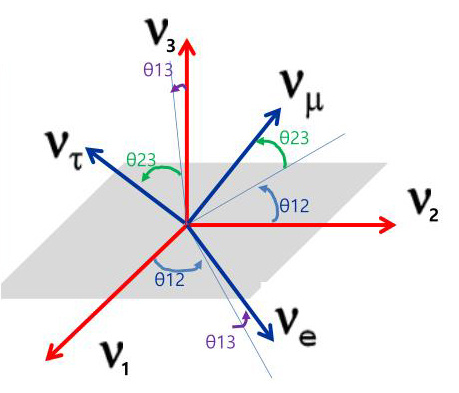
\includegraphics[width=0.4\linewidth]{basis.jpg}
  \caption{Reference rotation of the flavor basis versus the mass basis. The corresponding mixing angles are shown.}
  \label{fig:intro:basis}
\end{figure}

With rewriting equations~\autoref{eq:intro:app} and~\autoref{eq:intro:dis} with the new parametrization for the $\nu_e$ and $\nu_\mu$ will result

\begin{align}
P_{\nu_\mu\to\nu_\mu}=&1-\sin^22\theta_{23}\sin^2\frac{\Delta m^2_{13}L}{4E_\nu} \\
&+\left(\frac{1}{2}\cos^2\theta_{12}\sin^22\theta_{23}-\sin\theta_{13}\sin^2\theta_{23}\sin2\theta_{23}\sin2\theta_{12}\cos\delta\right)\times \nonumber \\
&\times\sin\frac{\Delta m^2_{12}L}{4E_\nu}\sin\frac{\Delta m^2_{13}L}{4E_\nu}  \nonumber \\
P_{\nu_\mu\to\nu_e}=&\sin^2\theta_{23}\sin^2 2\theta_{13}\sin^2\frac{\Delta m^2_{13}L}{4E_\nu}+\frac{1}{2}\sin2\theta_{23}\sin2\theta_{12}\cos^2\theta_{13}\sin\frac{\Delta m^2_{12}L}{2E_\nu} \times \\
\times & \sin\frac{\Delta m^2_{13}L}{2E_\nu}\cos\delta-\sin2\theta_{23}\sin2\theta_{13}\cos^2\theta_{13}\sin\theta_{13}\times\frac{\Delta m_{12}^2L}{2E_\nu}\sin^2\frac{\Delta m^2_{13}L}{4E_\nu}\sin\delta \nonumber
\end{align}

The visualization of the formulas above are provided on~\autoref{fig:intro:osc1}. The oscillation curves for each initial state ($e, \mu, \tau$) and two $E/L$ are shown. From such plot it's much easier to understand the meaning of the oscillation parameters. The mixing angles define oscillation amplitude and the mass difference define frequency.

\begin{figure}[!ht]
\centering
\begin{minipage}{0.4\linewidth}
  \centering
  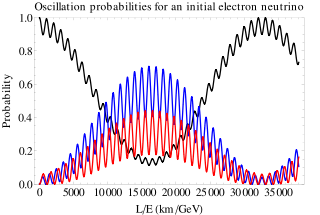
\includegraphics[width=\linewidth]{osc_ele_large.png}
\end{minipage}
\hfill
\begin{minipage}{0.4\linewidth}
  \centering
  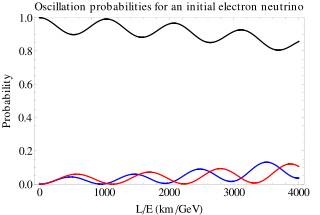
\includegraphics[width=\linewidth]{osc_ele_short.png}
\end{minipage}
\caption{Oscillation probabilities for the initial electron neutrino state for two different L/E scales. Black line corresponds to electron neutrino component, blue line for muon neutrino and red line for tau neutrino.}
\label{fig:intro:osc1}
\end{figure}

\begin{figure}
\centering
\begin{minipage}{0.4\linewidth}
  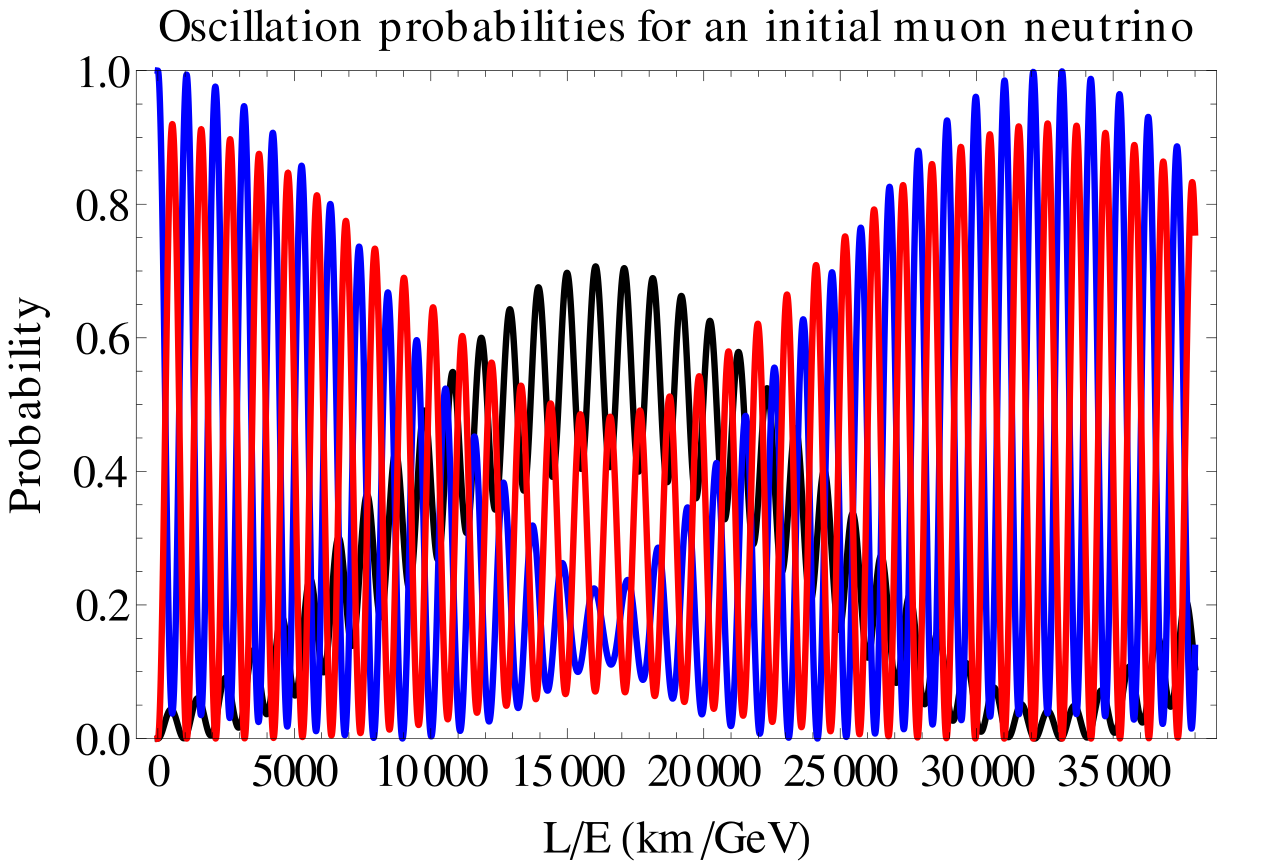
\includegraphics[width=\linewidth]{osc_muon_large.png}
\end{minipage}
\hfill
\begin{minipage}{0.4\linewidth}
  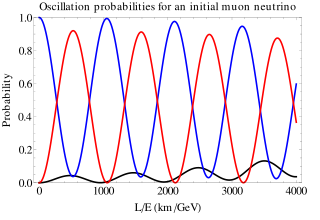
\includegraphics[width=\linewidth]{osc_muon_short.png}
\end{minipage}
\caption{Oscillation probabilities for the initial muon neutrino state for two different L/E scales. Black line corresponds to electron neutrino component, blue line for muon neutrino and red line for tau neutrino.}
\label{fig:intro:osc2}
\end{figure}

\begin{figure}
\centering
\begin{minipage}{0.4\linewidth}
  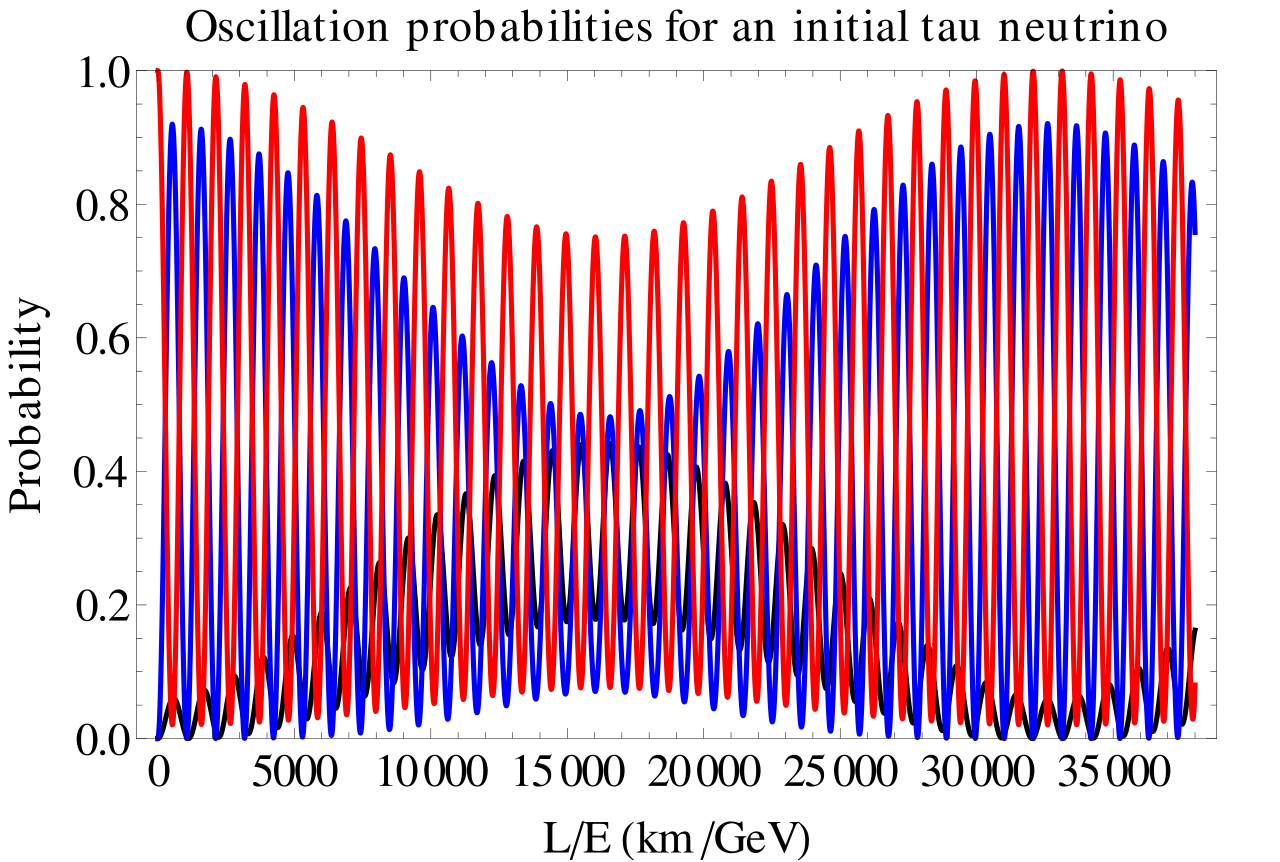
\includegraphics[width=\linewidth]{osc_tau_large.png}
\end{minipage}
\hfill
\begin{minipage}{0.4\linewidth}
  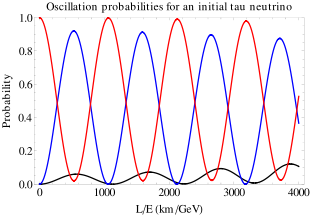
\includegraphics[width=\linewidth]{osc_tau_short.png}
\end{minipage}
\caption{Oscillation probabilities for the initial tau neutrino state for two different L/E scales. Black line corresponds to electron neutrino component, blue line for muon neutrino and red line for tau neutrino.}
\label{fig:intro:osc3}
\end{figure}


\subsubsection{2--flavor oscillations}
In the previous section the modern framework of the neutrino oscillations were described. Historically the neutrino mixing theory was developed for 2 flavors. While 3-flavor oscillation probability equations are quite complicated, a 2--flavor approximation often provides sufficient accuracy. In this approach the mixing matrix transforms to a usual 2x2 rotation matrix
\begin{equation}
U=
\begin{pmatrix}
\cos\theta    & \sin\theta     \\
-\sin\theta   & \cos\theta
\end{pmatrix}
\end{equation}
and the oscillation probabilities will be written as

\begin{align}
P_{\nu_\alpha\to\nu_\alpha}=1-&\sin^22\theta\sin^2\frac{1.27\Delta m^2L}{E_\nu} \\
P_{\nu_\alpha\to\nu_\beta}=&\sin^22\theta\sin^2\frac{1.27\Delta m^2L}{E_\nu}
\end{align}
in this notation the neutron energy unit is supposed to be GeV, the distance unit is km and the mass difference unit is $eV^2/c^2$.

\subsubsection{Oscillation in matter}
The framework presented above describes the oscillations in vacuum. In case of neutrino propagation in matter the effect will be different. Going through medium neutrino suffers from the forward elastic scattering with electrons and nucleons. This effect is similar to the phenomena of the light propagation in matter. The new potential which is equivalent to the refraction index, need to be taken into account. But the interaction types are slightly different for different neutrinos. All neutrino types may scatter over electrons, protons and neutrons through the neutral current exchange. In addition, electron neutrino scatters over the electrons with the charge current. The framework of the neutrino oscillations in mater was developed by Wolfenstein~\cite{Wolfenstein1978}. The mixing angle and the mass difference should be replaced by the effective ones, depending on the matter density.

Later it was discovered that in case of slightly changing density of the matter there is a region where the mixing angle reachs it's maximum possible value $\pi/4$~\cite{Mikheyev1985}. This phenomena is called Mikheyev–Smirnov–Wolfenstein (MSW) effect.

It's interesting to notice that non-zero mass difference is not necessary for the neutrino oscillations in matter. The flavor change is observable even in case of $\Delta m=0$ only because of the non-zero mixing angles~\cite{Smirnov2016}.


\subsubsection{Modern neutrino oscillation understanding}
In spite of the clear explanation of the neutrino oscillation phenomena within the quantum mechanics framework (\autoref{sec:osc}), this method suffers from incompleteness. For instance the assumption of the same momentum (or the same energy) of the different eigenstates is quite strong, but fully empirical. Also the normalization of the transition amplitude is not properly justified.

Another approach could solve some of the problems above. In case of the neutrino description only as a propagator between production and detection point (QFT framework) the normalization and all the conservation laws will come out of the box without manual tuning~\cite{Akhmedov2010a}.

Another interesting notice refers to the charge lepton oscillation problem. For instance mixing in the quark sector involves all the 9 quarks, while the oscillations in the lepton sector are usually notated as ``neutrino oscillations'' that affects only 3 uncharged leptons. In fact Pontecorvo-Maki-Nagava-Sakata matrix affects also charge leptons. But the coherence will be imminently ruined when the macroscopic sizes of source and detector are taken into account~\cite{Akhmedov2007}.

\subsection{Experiment overview}
\label{sec:exp}

\section{Prospects of the neutrino physics}



\chapter{HNL analysis motivation}
\label{ch:intro:HNL}

As presented in the \autoref{sec:osc} of~\autoref{ch:nu_phys} during the exploration of the neutrino oscillation phenomenon, non-zero difference between neutrino eigenstates was observed. That leads to the conclusion that at least two of the three eigenstates should be massive. While in the SM the neutrinos are massless (\autoref{sec:sm} of ~\autoref{ch:nu_phys}). The theory explaining the mass origin of the neutrino is required.

The easiest solution is try to implement the same process that gives mass to all other particles in the SM --- Higgs mechanism~\cite{Higgs1964} (also called Englert–Brout–Higgs–Guralnik–Hagen–Kibble mechanism for all contributed scientists). There are several problems on this way:
\begin{itemize}
  \item the scale of the neutrino mass is very different from the other particles in the SM. The neutrino masses are less then 1 eV~\cite{Aker2019}, while the other particles masses are $\gtrsim 1$ MeV, that gives us a difference of at least 6 orders. It could be event larger up to 8 orders in case of minimum possible neutrino mass. It's hard to believe that the same mechanism is responsible of the generation of mass at so different scales.
  \item as described in the~\autoref{sec:anti} only left-handed neutrinos and right-handed anti-neutrinos were observed. While for the Higgs mechanism both left and right handed particles are required.
\end{itemize}

That leads to the fact that we need to implement some new mechanism or/and new fundamental particles to explain the origin of the neutrino masses.

\section{Theory}
In this section the main models of neutrino mass generation will be overviewed. Dirac and Majorana mass terms will be presented as well as a ``mixed'' model of merging this two approaches (seesaw mechanism).

\subsection{Dirac mass term}
In the Standard Model of the particle physics the mass all the particles is generated with the Higgs mechanism. For example the Higgs-lepton Yukawa Lagrangian provides a natural explanation for the masses for the charged leptons
\begin{equation}
\mathcal{L}_{H, L}=-\sum_{\alpha, \beta=e,\mu,\tau}Y'^\ell_{\alpha\beta}\overline{L'_{\alpha L}}\Phi\ell'_{\beta R}+h.c
\end{equation}
Applying the same approach for the neutrino mass generation we will get the Lagrangian
\begin{align}
\mathcal{L}&=-\sum_{\alpha\beta=e,\mu,\tau}\bar{\nu}_{L,\alpha}(m_D)_{\alpha\beta}\nu_{R,\beta}+h.c. =\nonumber \\
&=-\overline{\nu_L}m_D\nu_R+h.c.
\end{align}
where $m_D$ is a 3x3 complex matrix. It could be diagonalized $m_D=U^\dag m V$, where U and V are unitary and $m_i\delta_{ik}$, $m_i>0$. After digitalization we could separate

\begin{align}
\nu_{\alpha L}&=\sum_iU_{\alpha i}\nu_{iL} \nonumber \\
\nu_{\alpha R}&=\sum_iV_{\alpha i}\nu_{iR}
\end{align}
and define $\nu\equiv\nu_L+\nu_R$. Thus the Dirac mass term will be expressed as
\begin{equation}
\label{eq:intro:dirac}
\mathcal{L}^{D}_{mass}=-\sum_im_i\overline{\nu_i}\nu_i
\end{equation}
where $\nu_i$, $i=1, 2, 3$ are neutrino mass eigenstates and $\nu_{\alpha L}$ are left-handed neutrino flavor eigenstate. The transition between them is defined with PMNS matrix (\autoref{eq:intro:mixing}).

\subsection{Majorana mass term}
As mentioned in the~\autoref{sec:anti} neutrino could be described with the Majorana equation in case $\psi=\psi^C$. To generate the mass for such a particle we need only one chiral fermion field. As neutrino is left-handed let us notate is at $\nu_L$. To write the mass term for this specific case we need to use $\nu_L$ alone. Modifying~\autoref{eq:intro:dirac}
\begin{equation}
\mathcal{L}^D_{mass}=-m\overline{\nu}\nu=-m\left(\overline{\nu_R}\nu_L+\overline{\nu_L}\nu_R\right)=-m\overline{\nu_R}\nu_L+h.c.
\end{equation}

Here $\nu_R$ should be replaced with right-handed function of the $\nu_L$. in fact it's a charge conjugated field
\begin{equation}
\nu_L^C=\mathcal{C}\overline{\nu_L}^T
\end{equation}
Thus the Majorana mass term could be expressed as
\begin{equation}
\mathcal{L}^M_{mass}=-\frac{1}{2}m\overline{\nu_L^C}\nu_L+h.c.
\end{equation}

The Majorana mass term provides an interesting mechanism of the generation of the neutrino mass. But it implements also physics beyond the SM. The lepton number is an invariant in the SM because of the U(1) symmetry. With the Majorana model it there is no such symmetry anymore. This leeds to the processes when the lepton number is violated, e.g. neutrino-less double beta decay.

Also such theory contains a product of fields with energy dimensions five


\subsection{Mixing Dirac and Majorana terms}
The most perspective approach is a combination the both Dirac and Majorana terms. In this case the model is very flexible and could provide the natural explanation of the neutrino masses with minimum extensions over the Standard Model. The mass term will be written with
\begin{equation}
\label{eq:intro:comb}
\mathcal{L}_{mass}^{D+M}=\mathcal{L}^D_{mass}+\mathcal{L}^R_{mass}+\mathcal{L}^L_{mass}
\end{equation}
where
\begin{align}
\mathcal{L}^L_{mass}&=\frac{1}{2}\sum_{\alpha,\beta}\nu'^T_{\alpha L}\mathcal{C}^\dagger M^L_{\alpha\beta}\nu'_{\beta L}+h.c. \\
\mathcal{L}^R_{mass}&=\frac{1}{2}\sum_{s, s'}\nu^T_{s R}\mathcal{C}^\dagger M^R_{ss'}\nu'_{s' R}+h.c. \\
\mathcal{L}^D_{mass}&=-\sum_{s=s_1, ..., s_{N_s}}\sum{\alpha}\overline{\nu_{sR}}M^D_{ss'}\nu'_{\alpha L} +h.c.
\end{align}

In the equations above the Greek indexes as usual corresponds to the flavor states, L and R illustrate the chirality and $s_i$ describes the sterile neutrino types. Thus matrix $M^L$ will be symmetric 3x3, $M^R$ --- symmetric $N_s\times N_x$ and $M^D$ --- $N_s\times3$. The mass matrix for the some of this three components will be written with
\begin{equation}
M^{D+M}\equiv
\begin{pmatrix}
M^L & {M^D}^T \\
M^D & M^R
\end{pmatrix}
\end{equation}

and the mass states will be presented with

\begin{align}
\nu_R^C\equiv
\begin{pmatrix}
\nu^C_{s_1R} \\
\vdots \\
\nu^C_{s_{N_S}R}
\end{pmatrix}
&&
N'_L\equiv
\begin{pmatrix}
\nu'_L \\ \nu^C_R
\end{pmatrix}
\end{align}

And the mass term~\autoref{eq:intro:comb} with new noteations will be rewritten as
\begin{equation}
\mathcal{L}_{mass}^{D+M}=\frac{1}{2}N'^T\mathcal{C}^\dagger M^{D+M}N'_L+h.c.
\end{equation}

There are plenty ways to combine Dirac and Majorana terms. With different initial assumptions the theory result could be quite different. Here there are the main hypothesis. In the notation below $m_D$ describes the Dirac mass, $m_L$, $m_R$ describe Majorana mass and the $m_{1,2}$ describes the mass eigenstates observable in the experiment.
\begin{itemize}
  \item Maximal mixing. $m_L=m_R$, $m_{2, 1}=m_L\pm m_D$, $\Delta m^2=m_2^2-m_1^2=4m_L m_D$
  \item Dirac limit. $m_L=m_R=0$, $m_{2,1}=\pm m_D$
  \item Pseudo-Dirac neutrinos. $\left|m_L\right|,m_R \ll m_D$, $m_{2,1}\approx\frac{m_L+m_R}{2}\pm m_D$
  \item Seesaw mechanism. $m_D \ll m_R$, $m_L=0$
\end{itemize}

\subsubsection{Seesaw mechanism}
Among all of the theories with Dirac and Majorana mixing the seesaw mechanism seems to be the most perspective. Here are the main advantages of this hypothesis:
\begin{itemize}
  \item The gauge symmetry is not broken as $m_L=0$
  \item The only ``exotic'' part (Sm extension) is implementation of $m_R$
  \item The Dirac mass could be easily explained with the Higgs method as $m_D$ is close to the mass of the SM particles
  \item Tiny mass of the observed neutrino eigenstates could be described with mixing
\end{itemize}

So, how could we explain the fact that observed neutrino mass is so small? $m_D$ is generated with a Higgs mechanism and could be GeV scale. $m_R$ is an exotic part of the theory. As it is a Majorana term it will violate the lepton number. But it will take place only at extremely high energies, much more then electroweak scale. The observed neutrino mass will be given by the mixing:
\begin{align}
m_1\approx\frac{m_D^2}{m_R} \ll m_D && m_2\approx m_R \gg m_D
\end{align}

and the mixing angle will be set as

\begin{equation}
\theta\approx\frac{m_D}{m_R} \ll 1
\end{equation}

For example, imagine the Dirac mass is fixed with $m_D=170 GeV$ and observed neutrino mass $m_1=5\times 10^-2 eV$, then the Majorana mass will be at the extremely high energy scale $M_R\approx10^{15}GeV$.



\section{Experiments and challenges}

\end{document}